\begin{center}
{\textbf{Jeudi 19 août 2021 : Veille de l’entraînement}}
\end{center}
\vspace{2mm}

Sans que l’on s’en soit aperçu, on est déjà presque arrivé à la moitié du stage ! Il va bientôt être temps de prendre un peu de repos. Mais, en attendant, on apporte les dernières touches au contenu mathématique de la première partie du séjour.

9h. Les groupes A et B doivent à présent appliquer toutes leurs nouvelles connaissances en géométrie dans un TD avec Raphaël et Aurélien respectivement. Les élèves du groupe C assiste à leur dernier cours d’arithmétique du séjour avec Arthur. Martin et Alexander entraînent les membres du groupe D en inégalités.

13 h 30. Cette fois-ci, c’est aux groupes A et B de se heurter aux inégalités avec Auguste et Victor. Combinatoire avec Anna dans le groupe C, et arithmétique dans le groupe D avec Rémi et Pierre -Marie.

L’après-midi, les diverses activités sportives et ludiques continuent. Courses, volley, piscine, foot, jeux de sociétés…

\begin{figure}[H]
\centering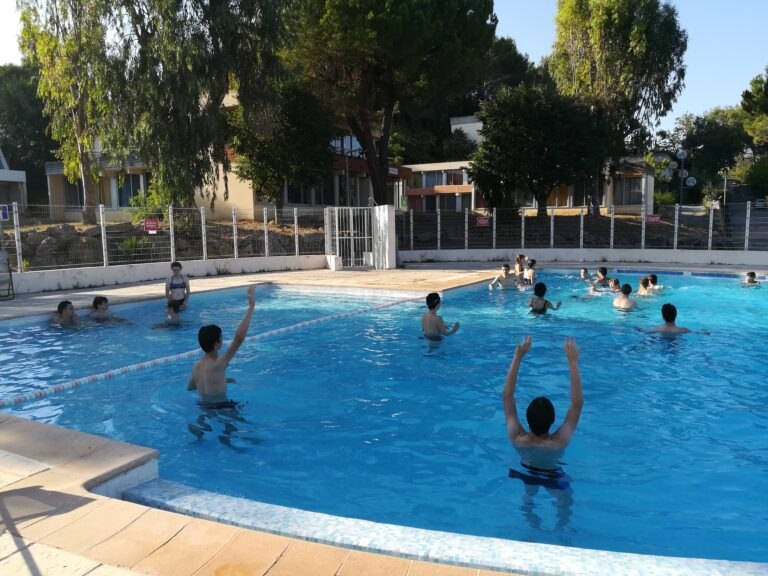
\includegraphics[height=7cm]{CR-19-0.jpg}\hspace{2cm}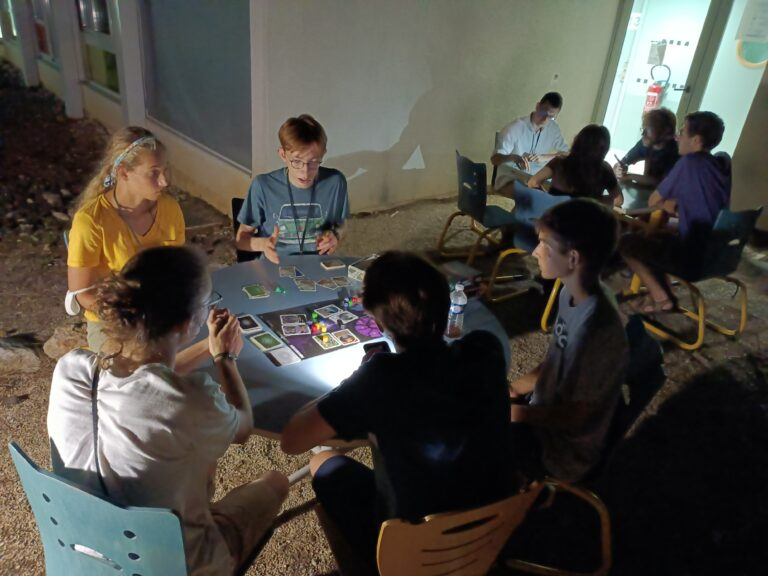
\includegraphics[height=7cm]{CR-19-1.jpg}
\caption{L’eau tiède ne refroidit pas l’enthousiasme des baigneurs. Une partie de jeux de balles ne tarde pas de s’organiser. Le soir, quel air d’insouciance ! S’ils savaient l'activité intellectuelle acharnée qui se déroule en salle anim pendant ce temps…}
\end{figure}

Hormis le stage olympique de mathématiques, le CIV accueille aussi d’autres évènements et rassemblements : stages de judo, chorales d’enfants et cette année : une convention nationale de science-fiction ! Pour quelques jours, le grand Hall de l’agora se remplit de stands avec livres et T-shirts thématiques.

Et, surprise, les initiés offrent, le temps d’une soirée, la possibilité à une quinzaine d’élèves d’infiltrer leurs rangs et participer à une conférence sur la physique dans la science-fiction à 18h.

Il n’y a pas de présentation la veille de l’entraînement de demain. Pas besoin de se faire de soucis pour les élèves tout autant : ces derniers savent parfaitement comment s’occuper.